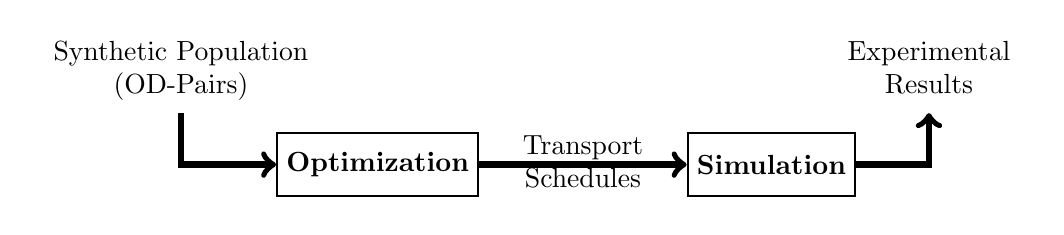
\begin{tikzpicture}
  \node (opt) at (0,0) [draw,thick,minimum height=0.8cm] {\bf Optimization};
  \node (sim) at (5,0) [draw,thick,minimum height=0.8cm] {\bf Simulation};
  \node (pop) at (-2.5, 1.2)  {\begin{tabular}{c}Synthetic Population \\ (OD-Pairs) \end{tabular} };
  \node (res) at (7, 1.2)  {\begin{tabular}{c}Experimental \\ Results \end{tabular} };
  \draw[->,line width=0.8mm] (opt) -- (sim)  node [midway,align=center]{\begin{tabular}{c}Transport \\ Schedules \end{tabular}}  ;
  \draw[->,line width=0.8mm]  (pop) -- (-2.5,0)  -- (opt);
  \draw[->,line width=0.8mm]  (sim) -- (7,0)  -- (res);
\end{tikzpicture}
